\documentclass{beamer}
\usepackage[latin9]{inputenc}
\usepackage{unicode}
\usepackage{hyperref}
\usepackage[austrian]{babel}
\usepackage[T1]{fontenc}
\usepackage[round]{natbib}
\usepackage{graphicx}
\usepackage{C:/Programme/R/share/texmf/Sweave}
\usepackage{beamerthemesplit} % kam neu dazu


\begin{document}
\title{\textbf{Sch�tzung und Kalibrierung von Copulae}\\
  \emph{Welche Copula passt zu meinen Daten?} \\
  \footnotesize{Implementierung von Sch�tzungsmethoden f\"ur den
    bivariaten Fall in 
    \emph{R}}
}

\author{
  Gerold K�b (0250001)\\
  Martin Gartner (0351427)
}
\date{\today} 



%%%%%%%%%%%%%%%%%%%%%%%%%%%%%%%%%%%%%%%%%%%%%%%%%%%%%%%%%%%%%%%%%%%%%%
%%%%%%%%%%%%%%%%%%%%%%%%%%%%%%%%%%%%%%%%%%%%%%%%%%%%%%%%%%%%%%%%%%%%%%
%%%%%%%%%%%%%%%%%%%%%%%%%%%%%%%%%%%%%%%%%%%%%%%%%%%%%%%%%%%%%%%%%%%%%%

\frame{\titlepage} 
\frame{\frametitle{Inhaltsverzeichnis}\footnotesize{\tableofcontents}}

\section{Warum Copulae verwenden?}
% \subsection{Motivation} 
\frame{\frametitle{Motivation} 
  Finanzm�rkte der Realit�t entsprechen h�ufig nicht den Annahmen der
  Finanzmarkttheorie, zB 

  \begin{itemize}
  \item \textit{fat tails} der Verteilungen
  \item Korrelation von null bedeutet in Praxis nicht zwingend
    Unabh�ngigkeit 
  \item Auftreten von Clustern in Volatilit�t
  \end{itemize}

  Dies f\"uhrt zu Schwierigkeiten im Sch�tzen der gemeinsamen
  Verteilungsfunktion eines Portfolios. 
}




% \subsection{Probleme gemeinsamer Verteilungsfunktionen}
\frame{\frametitle{Probleme gemeinsamer Verteilungsfunktionen}
  Probleme:
  \begin{itemize}
  \item Kann man VaR zweier Instrumente einfach addieren um VaR des
    Portfolios zu erhalten? 
  \item Wie kann man Abh�ngigkeit innerhalb der Instrumente des
    Portfolios beschreiben? 
  \item Pearson's Korrelation hat einige Nachteile
  \end{itemize}
  
  L�sung:
  \begin{itemize}
  \item Mit Copulae kann Abh�ngigkeitsstruktur und gemeinsame
    Verteilung besser gesch�tzt werden! 
  \end{itemize}  
}

%%%%%%%%%%%%%%%%%%%%%%%%%%%%%%%%%%%%%%%%%%%%%%%%%%%%%%%%%%%%%%%%%%%%%%
%%%%%%%%%%%%%%%%%%%%%%%%%%%%%%%%%%%%%%%%%%%%%%%%%%%%%%%%%%%%%%%%%%%%%%
%%%%%%%%%%%%%%%%%%%%%%%%%%%%%%%%%%%%%%%%%%%%%%%%%%%%%%%%%%%%%%%%%%%%%%

\section{Copulae}
\subsection{Was ist eine Copula?}
\frame{\frametitle{Was ist eine Copula?}
  Eine \emph{Copula} ist eine Funktion, die eine
  multivariate Verteilungsfunktion mit ihren eindimensionalen
  Randverteilungen kombiniert.

  \begin{itemize}
  \item $X$, $Y$ \ldots zwei stetige Zufallsvariablen mit $F(x)~=~P(X
    \leq x)$ und $G(y) = P(Y \leq y)$ 
  \item gemeinsame Verteilung $H(x, y) = P(X \leq x, Y \leq y)$
  \item f\"ur $(x, y)~\in~[-\infty, \infty]^2$ gibt es Punkt
    $\left(F(x), G(y), H(x,y)\right)$ 
  \item \emph{Copula} ist nun die Abbildung von $\mathbf{I}^2$ nach
    $\mathbf{I}$ 
  \end{itemize}
}

%%%%%%%%%%%%%%%%%%%%%%%%%%%%%%%%%%%%%%%%%%%%%%%%%%%%%%%%%%%%%%%%%%%%%%
%%%%%%%%%%%%%%%%%%%%%%%%%%%%%%%%%%%%%%%%%%%%%%%%%%%%%%%%%%%%%%%%%%%%%%
%%%%%%%%%%%%%%%%%%%%%%%%%%%%%%%%%%%%%%%%%%%%%%%%%%%%%%%%%%%%%%%%%%%%%%

\frame{\frametitle{Interpretation als Volumen}
  Darstellbar als Volumen in $\mathbf{I}^3$:
  \begin{figure}[htb]  
    \centering
    % \label{fig:copulabounds}
    % \caption{Frechet-Hoeffding-Bounds}
    \begin{minipage}[b]{.3\textwidth} % [b] => Ausrichtung an \caption
      \caption{$W(x, y)$}
      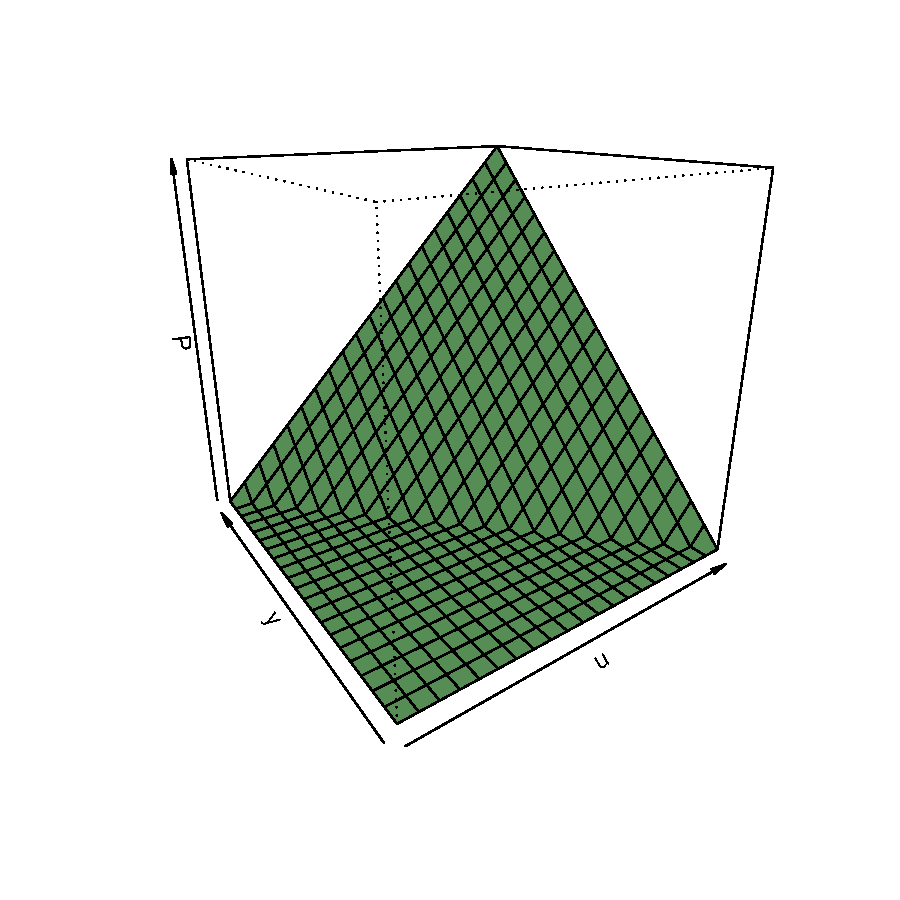
\includegraphics[width = \textwidth]{copulaM}
    \end{minipage}
    \hspace{.0\linewidth}% Abstand zwischen Bilder
    \begin{minipage}[b]{.3\textwidth} % [b] => Ausrichtung an \caption
      \caption{$\Pi(x, y)$}
      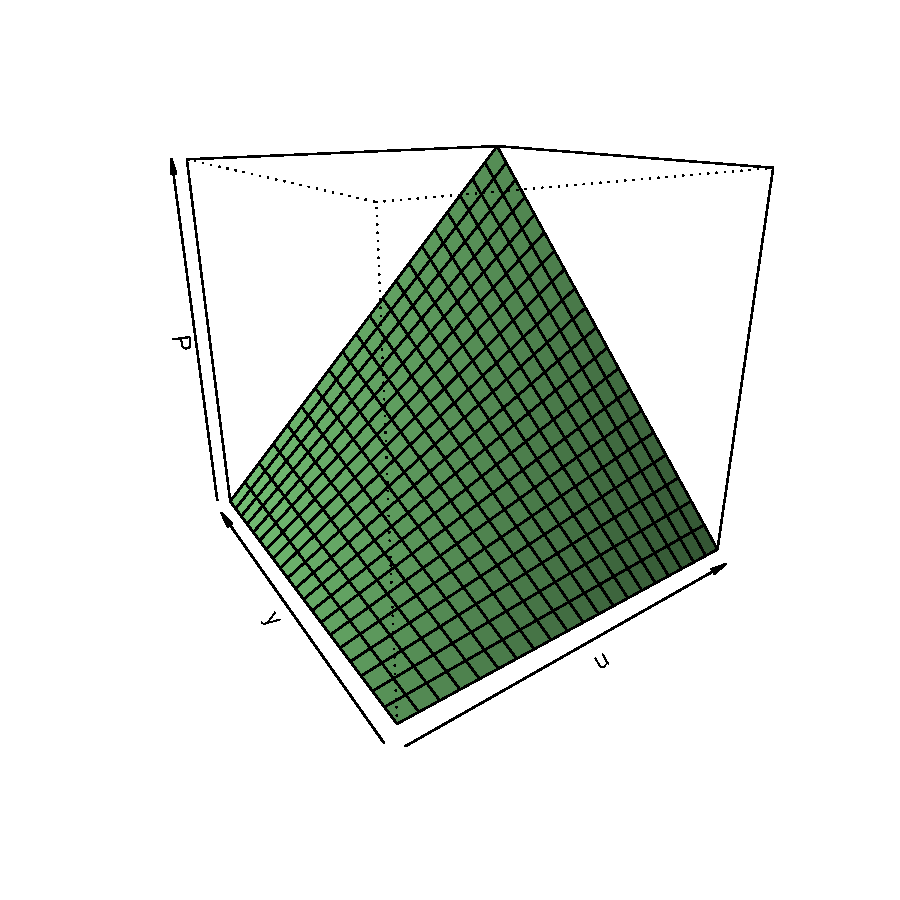
\includegraphics[width = \textwidth]{copulaPi}
    \end{minipage}
    \hspace{.0\linewidth}% Abstand zwischen Bilder
    \begin{minipage}[b]{.3\textwidth} % [b] => Ausrichtung an \caption
      \caption{$M(x, y)$}
      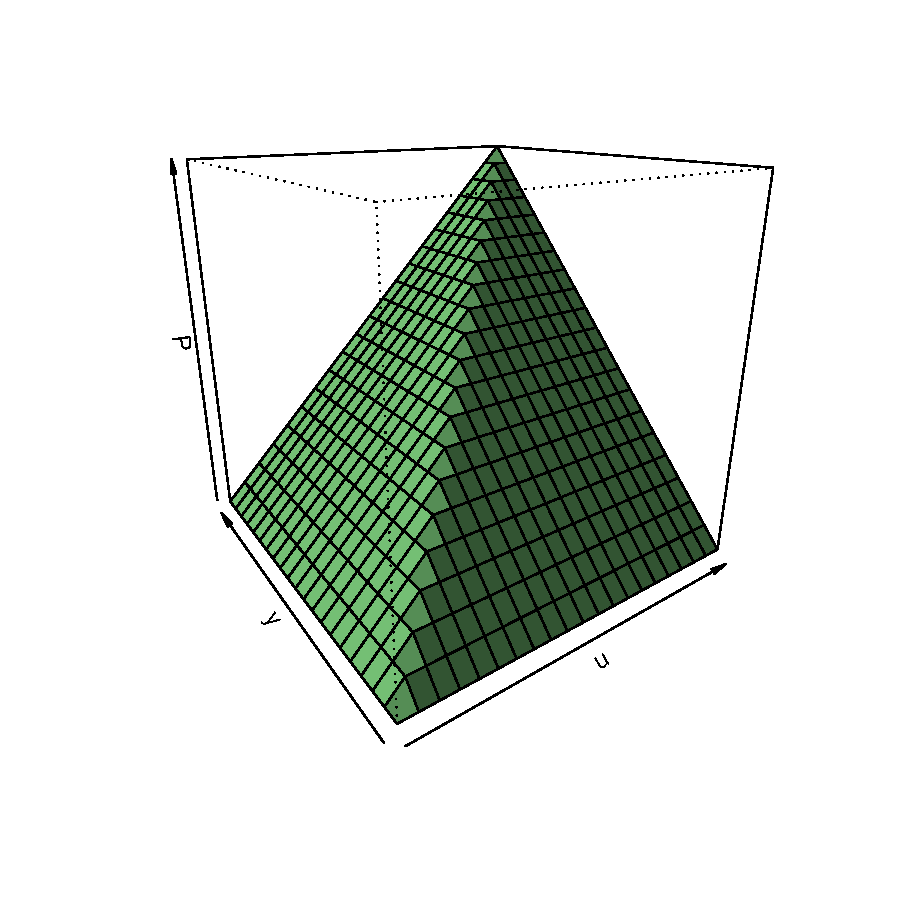
\includegraphics[width = \textwidth]{copulaW}
    \end{minipage}
  \end{figure}
  
  und daher als Wahrscheinlichkeitskennzahl in $\mathbf{I}^2$
  interpretierbar.
}

%%%%%%%%%%%%%%%%%%%%%%%%%%%%%%%%%%%%%%%%%%%%%%%%%%%%%%%%%%%%%%%%%%%%%%
%%%%%%%%%%%%%%%%%%%%%%%%%%%%%%%%%%%%%%%%%%%%%%%%%%%%%%%%%%%%%%%%%%%%%%
%%%%%%%%%%%%%%%%%%%%%%%%%%%%%%%%%%%%%%%%%%%%%%%%%%%%%%%%%%%%%%%%%%%%%%

\subsection{Sklar's Theorem}
\frame{\frametitle{Sklar's Theorem}
  Gemeinsame Verteilung kann durch die \emph{Copula} ausgedr\"uckt
  werden:
  \begin{equation}
    \label{eq:sklar}
    H(x, y) = C(F(x), G(y))
  \end{equation}
  Gilt auch f\"ur den multivariaten Fall!\\~\\
  
  Alle Copulae liegen zwischen zwei Grenzen. Seien $M$ und $W$ die
  Copulae
  \begin{eqnarray}
    \label{eq:bounds}
    M(x, y) & = & \min{(x, y)} \\
    W(x, y) & = & \max{ (x + y - 1, 0)}
  \end{eqnarray}
}

%%%%%%%%%%%%%%%%%%%%%%%%%%%%%%%%%%%%%%%%%%%%%%%%%%%%%%%%%%%%%%%%%%%%%%
%%%%%%%%%%%%%%%%%%%%%%%%%%%%%%%%%%%%%%%%%%%%%%%%%%%%%%%%%%%%%%%%%%%%%%
%%%%%%%%%%%%%%%%%%%%%%%%%%%%%%%%%%%%%%%%%%%%%%%%%%%%%%%%%%%%%%%%%%%%%%

\subsection{Die Frech\'et-Hoeffding Bounds}
\frame{\frametitle{Eigenschaften von Copulae}
  Es gilt
  \begin{equation}
    \label{eq:frechethoeffding}
    W(x, y) \leq C(x, y) \leq M(x, y)
  \end{equation}
  \begin{figure}[htb]  
    \centering
    % \label{fig:copulabounds}
    % \caption{Frechet-Hoeffding-Bounds}
    \begin{minipage}[b]{.3\textwidth} % [b] => Ausrichtung an \caption
      \caption{$W(x, y)$}
      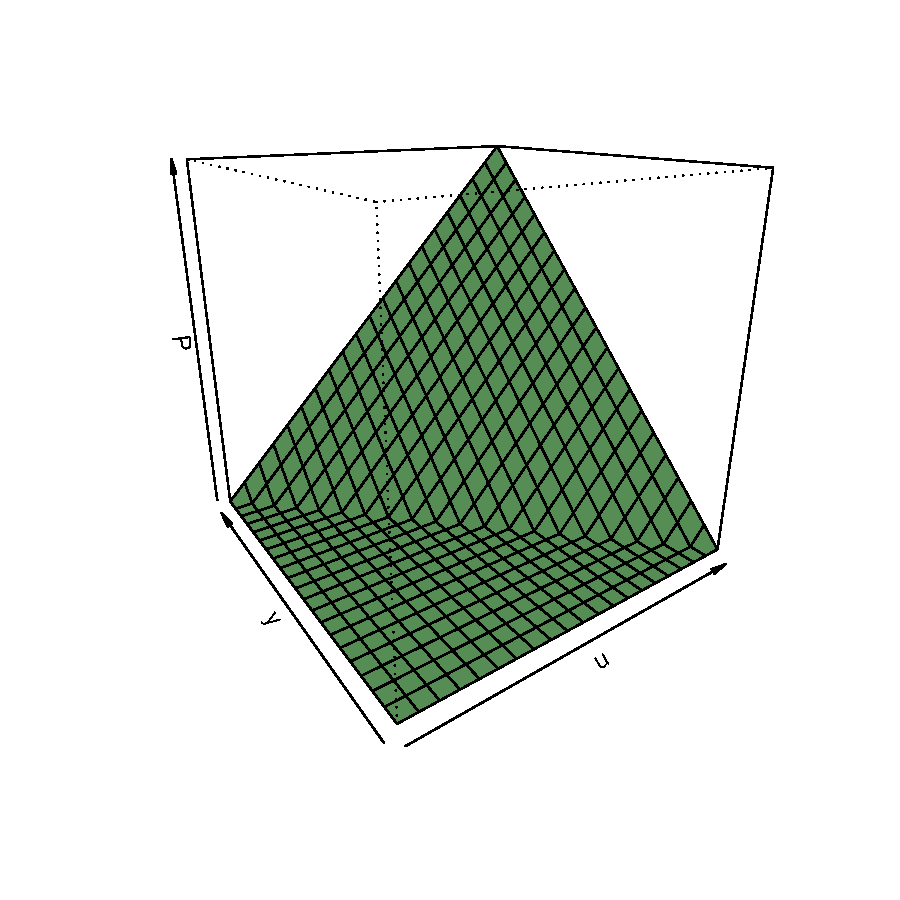
\includegraphics[width = \textwidth]{copulaM}
    \end{minipage}
    \hspace{.0\linewidth}% Abstand zwischen Bilder
    \begin{minipage}[b]{.3\textwidth} % [b] => Ausrichtung an \caption
      \caption{$\Pi(x, y)$}
      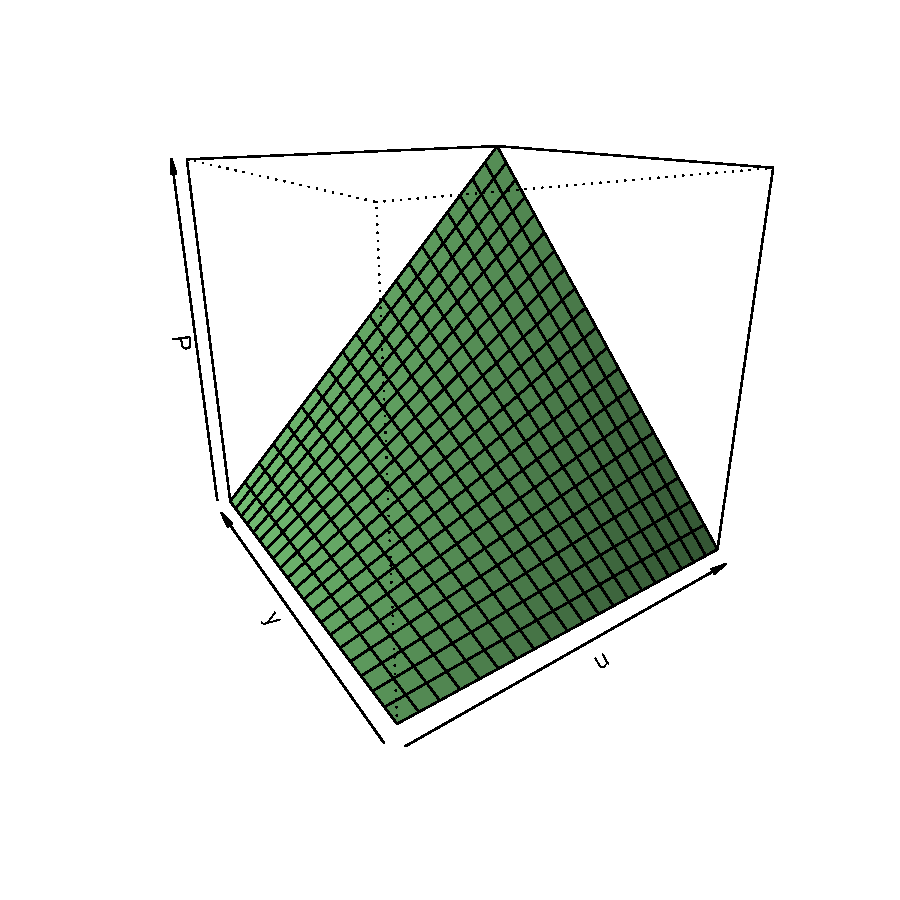
\includegraphics[width = \textwidth]{copulaPi}
    \end{minipage}
    \hspace{.0\linewidth}% Abstand zwischen Bilder
    \begin{minipage}[b]{.3\textwidth} % [b] => Ausrichtung an \caption
      \caption{$M(x, y)$}
      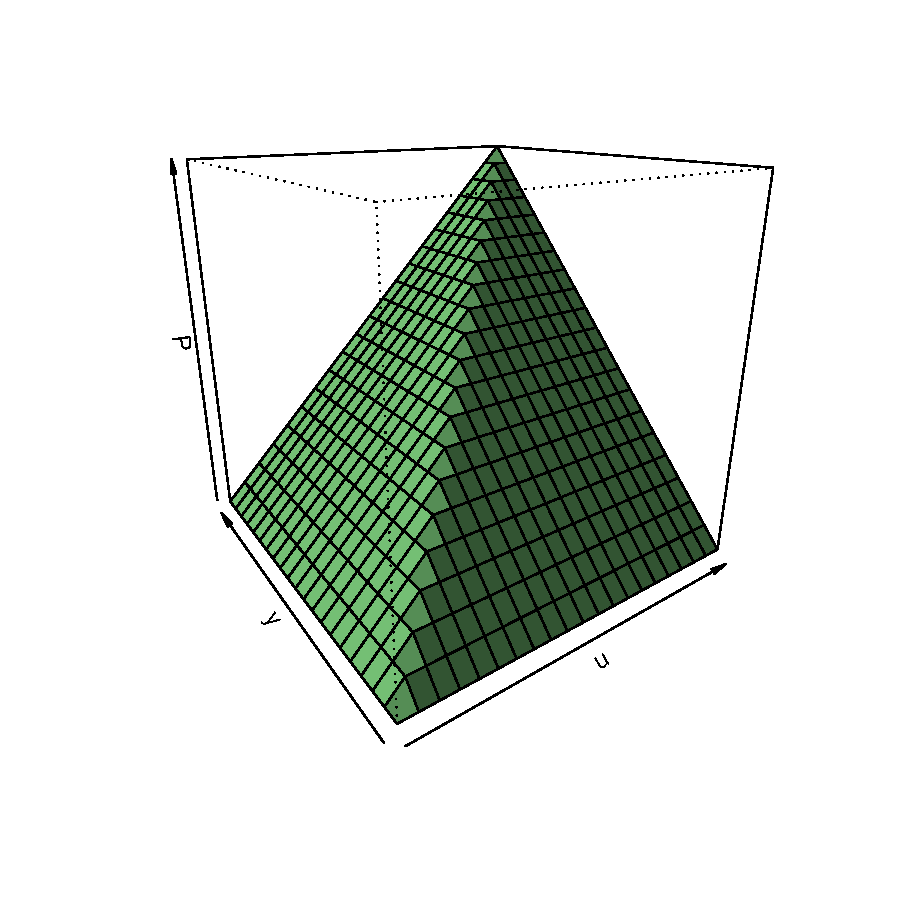
\includegraphics[width = \textwidth]{copulaW}
    \end{minipage}
  \end{figure}
}

%%%%%%%%%%%%%%%%%%%%%%%%%%%%%%%%%%%%%%%%%%%%%%%%%%%%%%%%%%%%%%%%%%%%%%
%%%%%%%%%%%%%%%%%%%%%%%%%%%%%%%%%%%%%%%%%%%%%%%%%%%%%%%%%%%%%%%%%%%%%%
%%%%%%%%%%%%%%%%%%%%%%%%%%%%%%%%%%%%%%%%%%%%%%%%%%%%%%%%%%%%%%%%%%%%%%

\section{Familien von Copulae}
\frame{\frametitle{Familien von Copulae}

  \begin{block}{Elliptische Copulae}
    \begin{itemize}
    \item Copulae von	elliptischen Verteilungen\
    \item zB beide Randverteilungen sind normal- oder t-verteilt
    \end{itemize}
  \end{block}

  \begin{block}{Archimedische Copulae}
    \begin{itemize}
    \item einfach zu erzeugen
    \item viele parametrische Familien (22 nach Nelsen (2006))
    \item k�nnen an viele gew\"unschte Eigenschaften angepasst
      werden
    \end{itemize}
  \end{block}
}

%%%%%%%%%%%%%%%%%%%%%%%%%%%%%%%%%%%%%%%%%%%%%%%%%%%%%%%%%%%%%%%%%%%%%%
%%%%%%%%%%%%%%%%%%%%%%%%%%%%%%%%%%%%%%%%%%%%%%%%%%%%%%%%%%%%%%%%%%%%%%
%%%%%%%%%%%%%%%%%%%%%%%%%%%%%%%%%%%%%%%%%%%%%%%%%%%%%%%%%%%%%%%%%%%%%%

\subsection{Elliptische Copulae}
\frame{\frametitle{Elliptische Copulae f\"ur n = 2}
  \begin{block}{Gau�'sche Copula}
    \small{
      \begin{equation}
        C_G(u,v) = \int_{-\infty}^{\Phi^{-1}(u)}
        \int_{-\infty}^{\Phi^{-1}(v)} \frac{1}{2 \pi \sqrt{(1 - \rho^2)}}
        \exp{ \left( -\frac{s^2 - 2 \rho s t + t^2} {2 (1 - \rho^2)}
          \right) }ds dt
      \end{equation}
    }
  \end{block}
  \begin{block}{T-Copula}
    \small{
      \begin{equation}
        C_t(u, v) = \int_{-\infty}^{t_{\nu}^{-1}(u)}
        \int_{-\infty}^{t_{\nu}^{-1}(v)} \frac{1}{2 \pi \sqrt{(1 - \rho^2)}}
        \exp{ \left( -\frac{s^2 - 2 \rho s t + t^2} {2 (1 - \rho^2)}
          \right) }ds dt
      \end{equation}
    }
  \end{block}
}

%%%%%%%%%%%%%%%%%%%%%%%%%%%%%%%%%%%%%%%%%%%%%%%%%%%%%%%%%%%%%%%%%%%%%%
%%%%%%%%%%%%%%%%%%%%%%%%%%%%%%%%%%%%%%%%%%%%%%%%%%%%%%%%%%%%%%%%%%%%%%
%%%%%%%%%%%%%%%%%%%%%%%%%%%%%%%%%%%%%%%%%%%%%%%%%%%%%%%%%%%%%%%%%%%%%%


\subsection{Archimedische Copulae}
\frame{\frametitle{Archimedische Copulae}
  \begin{block}{Eigenschaften:}
    \begin{itemize}
    \item k�nnen sehr einfach erzeugt werden
    \item viele parametrische Familien 
    \item besitzen viele gew\"unschte Eigenschaften
    \end{itemize}
  \end{block}

  \begin{block}{Einfachheit der Kostruktion:}
    
    Sei $\varphi$ 
    eine stetige und konvexe Funktion von $\mathbf{I}$ nach $[0, \infty]$,
    sodass $\varphi(1) = 0$ und $\varphi(0) = \infty$. Sei $\varphi^{[-1]}$ die
    Pseudo-Inverse von $\varphi$

    \begin{equation}
      \label{eq:archm}
      C(u, v) = \varphi^{[-1]}(\varphi(u) + \varphi(v))
    \end{equation}
  \end{block}
}

%%%%%%%%%%%%%%%%%%%%%%%%%%%%%%%%%%%%%%%%%%%%%%%%%%%%%%%%%%%%%%%%%%%%%%
%%%%%%%%%%%%%%%%%%%%%%%%%%%%%%%%%%%%%%%%%%%%%%%%%%%%%%%%%%%%%%%%%%%%%%
%%%%%%%%%%%%%%%%%%%%%%%%%%%%%%%%%%%%%%%%%%%%%%%%%%%%%%%%%%%%%%%%%%%%%%

\section{Fit-Methoden}
\frame{\frametitle{Fit-Methoden}
  \begin{block}{3 Methoden:}
  \begin{itemize}
  \item Exact Maximum Likelihood (EML) method (one stage method)
  \item Inference Functions for Margins (IFM) method (two stage method)
  \item Canonical Maximum Likelihood (CML) method
  \end{itemize}
  \end{block}
}

%%%%%%%%%%%%%%%%%%%%%%%%%%%%%%%%%%%%%%%%%%%%%%%%%%%%%%%%%%%%%%%%%%%%%%
%%%%%%%%%%%%%%%%%%%%%%%%%%%%%%%%%%%%%%%%%%%%%%%%%%%%%%%%%%%%%%%%%%%%%%
%%%%%%%%%%%%%%%%%%%%%%%%%%%%%%%%%%%%%%%%%%%%%%%%%%%%%%%%%%%%%%%%%%%%%%


\subsection{Exact Maximum Likelihood (EML) method}
\frame{\frametitle{Exact Maximum Likelihood (EML) method}
  \begin{itemize}
  \item Versucht Parameter der Randverteilung und der Copula gleichzeitig zu
    sch�tzen.  
  \item $\theta$ steht f\"ur Vektor mit allen Parametern
  \end{itemize}
\begin{equation}
    \label{eq:EML}
    l(\theta) = \sum^{T}_{t=1} \ln c(F_1(x_{1t}),...,F_n(x_{nt})) +
    \sum^{T}_{t=1}\sum^{n}_{j=1} \ln  f_j(x_{jt})
  \end{equation}
}

%%%%%%%%%%%%%%%%%%%%%%%%%%%%%%%%%%%%%%%%%%%%%%%%%%%%%%%%%%%%%%%%%%%%%%
%%%%%%%%%%%%%%%%%%%%%%%%%%%%%%%%%%%%%%%%%%%%%%%%%%%%%%%%%%%%%%%%%%%%%%
%%%%%%%%%%%%%%%%%%%%%%%%%%%%%%%%%%%%%%%%%%%%%%%%%%%%%%%%%%%%%%%%%%%%%%

\subsection{Inference Functions for Margins (IFM) method}
\frame{\frametitle{Inference Functions for Margins (IFM) method}
  \begin{itemize}
  \item 1. Schritt: Sch�tzen der Parameter  der Randverteilungen
    $\theta_1$ und $\theta_2$ mit ML-Methode     
  \item 2. Schritt: Sch�tzen der Parameter der Copula (angepasste
    Randverteilungen bereits durch Schritt 1 gegeben)
  \end{itemize}

  \begin{equation}
    \label{eq:IFMcopula}
    \hat{\theta}_{2} = \arg\max_{\theta_2} \sum^{T}_{t=1} \ln
    {c(F_1(x_{1t}),...,F_n(x_{nt});\theta_1,\hat{\theta}_{1})}
  \end{equation}
}

%%%%%%%%%%%%%%%%%%%%%%%%%%%%%%%%%%%%%%%%%%%%%%%%%%%%%%%%%%%%%%%%%%%%%%
%%%%%%%%%%%%%%%%%%%%%%%%%%%%%%%%%%%%%%%%%%%%%%%%%%%%%%%%%%%%%%%%%%%%%%
%%%%%%%%%%%%%%%%%%%%%%%%%%%%%%%%%%%%%%%%%%%%%%%%%%%%%%%%%%%%%%%%%%%%%%

\subsection{Canonical Maximum Likelihood (CML) method}
\frame{\frametitle{Canonical Maximum Likelihood (CML) method}
  \begin{itemize}
  \item 1. Schritt: Berechnung der empirischen Verteilungsfunktion
  \item 2. Schritt: Sch�tzen der Parameter der Copula mittels
    ML-Methode, wobei Werte der
    empirischen Verteilungsfunktion verwendet werden
  \end{itemize}
  \begin{equation}
    \label{eq:CML}
    \hat{\theta}_{2} = \arg \max_{\theta_2} \sum^{T}_{t=1} \ln
    c(\hat{F_1}(x_{1t}),...,\hat{F_n}(x_{nt});\theta_1,\hat{\theta}_{2})   
  \end{equation}
}

%%%%%%%%%%%%%%%%%%%%%%%%%%%%%%%%%%%%%%%%%%%%%%%%%%%%%%%%%%%%%%%%%%%%%%
%%%%%%%%%%%%%%%%%%%%%%%%%%%%%%%%%%%%%%%%%%%%%%%%%%%%%%%%%%%%%%%%%%%%%%
%%%%%%%%%%%%%%%%%%%%%%%%%%%%%%%%%%%%%%%%%%%%%%%%%%%%%%%%%%%%%%%%%%%%%%

\subsection{Vor- und Nachteile}
\frame{\frametitle{Vor- und Nachteile der einzelenen Methoden}
  \begin{block}{EML-Methode:}
    \begin{itemize}
    \item schwierig, weil Randverteilungen unterschiedlich viele
      Parameter besitzen k�nnen
    \item Parameter m\"ussen sowohl in Dichtefunktion der Copula und
      den Randverteilungen verwendet werden und \"ubereinstimmen
    \item AIC - hoher Strafterm
    \item lange Rechenzeit (viele Parameter werden gleichzeitig gesch�tzt)
    \end{itemize}
  \end{block}
}

%%%%%%%%%%%%%%%%%%%%%%%%%%%%%%%%%%%%%%%%%%%%%%%%%%%%%%%%%%%%%%%%%%%%%%
%%%%%%%%%%%%%%%%%%%%%%%%%%%%%%%%%%%%%%%%%%%%%%%%%%%%%%%%%%%%%%%%%%%%%%
%%%%%%%%%%%%%%%%%%%%%%%%%%%%%%%%%%%%%%%%%%%%%%%%%%%%%%%%%%%%%%%%%%%%%%

\frame{\frametitle{Vor- und Nachteile der einzelenen Methoden}
  \begin{block}{IFM-Methode:}
    \begin{itemize}
    \item einfach, schnell
    \item flexibel (viele Randverteilungen k�nnen verwendet werden)
    \item AIC - m�glicherweise verf�lscht, weil zweistufiger
      Optimierungsprozess 
    \end{itemize}    
  \end{block}

  \begin{block}{CML-Methode:}
  \begin{itemize}
  \item einfach, schnell
  \item unabh�ngig vom Aussehen der Randverteilungen
  \end{itemize}
  \end{block}

}

%%%%%%%%%%%%%%%%%%%%%%%%%%%%%%%%%%%%%%%%%%%%%%%%%%%%%%%%%%%%%%%%%%%%%%
%%%%%%%%%%%%%%%%%%%%%%%%%%%%%%%%%%%%%%%%%%%%%%%%%%%%%%%%%%%%%%%%%%%%%%
%%%%%%%%%%%%%%%%%%%%%%%%%%%%%%%%%%%%%%%%%%%%%%%%%%%%%%%%%%%%%%%%%%%%%%

\section{Beispiel}
\subsection{IFM-Methode}
\begin{frame}[containsverbatim]
  \frametitle{Fitten eines Beispieldatensatzes:}
  2 Zeitreihen: ATX und NIKKEI
\footnotesize{
\begin{Schunk}
\begin{Sinput}
> head(x)
\end{Sinput}
\begin{Soutput}
[1] 0.0005277 0.0041850 0.0031730 0.0124600 0.0040900 0.0090880
\end{Soutput}
\begin{Sinput}
> head(y)
\end{Sinput}
\begin{Soutput}
[1] -0.013890 -0.035990  0.003096  0.003390  0.008382 -0.001205
\end{Soutput}
\end{Schunk}
}

\normalsize{
Fit nach der IFM-Methode
}
\footnotesize{
\begin{Schunk}
\begin{Sinput}
> ifm <- CopulaFit(x, y, method = "IFM", returns = TRUE)
\end{Sinput}
\end{Schunk}
}
\end{frame}


\begin{frame}[containsverbatim]
  \frametitle{Ergebnisse IFM-Methode:}
\scriptsize{
\begin{Schunk}
\begin{Sinput}
> ifm
\end{Sinput}
\begin{Soutput}
   fit.family      fit.par fit.objective fit.method fit.convergence  fit.AIC
1    Archm. 1 -0.008746649 -9.037212e-05        IFM               0 1.999819
2    Archm. 3  0.050244838 -1.053455e-04        IFM               0 1.999789
3    Archm. 4  1.000000000 -1.463821e-17        IFM               0 2.000000
4    Archm. 5  0.102855182 -1.063884e-04        IFM               0 1.999787
5    Archm. 6  1.000000000  8.649854e-18        IFM               0 2.000000
6    Archm. 9  0.000000000  0.000000e+00        IFM               0 2.000000
7   Archm. 10  0.000000000  0.000000e+00        IFM               0 2.000000
8   Archm. 12  1.000000000  2.984621e-01        IFM               0 2.596924
9   Archm. 13  1.006500421 -3.669076e-06        IFM               0 1.999993
10  Archm. 14  1.000000000  2.984621e-01        IFM               0 2.596924
11  Archm. 16  0.198681184  2.020869e-01        IFM               0 2.404174
12  Archm. 17 -0.837100820 -8.937913e-05        IFM               0 1.999821
\end{Soutput}
\end{Schunk}
}
\end{frame}

\begin{frame}[containsverbatim]
  \frametitle{S3-Objekte:}
\scriptsize{
\begin{Schunk}
\begin{Sinput}
> attributes(ifm)
\end{Sinput}
\begin{Soutput}
$names
 [1] "margin1"      "distrmargin1" "margin2"      "distrmargin2" "family"      
 [6] "par"          "objective"    "AIC"          "convergence"  "message"     
[11] "iterations"   "method"      

$class
[1] "mloutput"
\end{Soutput}
\begin{Sinput}
> ifm$distrmargin2
\end{Sinput}
\begin{Soutput}
[1] "Normal Distribution"
\end{Soutput}
\begin{Sinput}
> ifm$margin2
\end{Sinput}
\begin{Soutput}
[1] -0.0002036121  0.0146507741
\end{Soutput}
\end{Schunk}
}

\end{frame}

\begin{frame}[containsverbatim]
  \frametitle{Summary IFM-Methode:}

\scriptsize{
\begin{Schunk}
\begin{Sinput}
> summary(ifm)
\end{Sinput}
\begin{Soutput}
 Die best-fit Copula ist Typ:  Archm. 5 
 Minimaler Zielfunktionswert:  -0.0001063884 

Summary:
  a.family.ind. a.objective.ind. a.method.ind.   a.par.ind. a.AIC.ind.
1      Archm. 5    -1.063884e-04           IFM  0.102855182   1.999787
2      Archm. 3    -1.053455e-04           IFM  0.050244838   1.999789
3      Archm. 1    -9.037212e-05           IFM -0.008746649   1.999819
  a.convergence.ind.
1                  0
2                  0
3                  0
\end{Soutput}
\end{Schunk}
}
\end{frame}

\subsection{Vergleich mit anderen Methoden}
\begin{frame}[containsverbatim]
  \frametitle{Vergleich CML-Methode:}
\scriptsize{
\begin{Schunk}
\begin{Sinput}
> summary(cml)
\end{Sinput}
\begin{Soutput}
 Die best-fit Copula ist Typ:  Archm. 5 
 Minimaler Zielfunktionswert:  -0.0001179483 

Summary:
  a.family.ind. a.objective.ind. a.method.ind.  a.par.ind. a.AIC.ind.
1      Archm. 5    -0.0001179483           CML  0.09181627   1.999764
2      Archm. 3    -0.0001178839           CML  0.04533770   1.999764
3     Archm. 17    -0.0001069186           CML -0.84801622   1.999786
  a.convergence.ind.
1                  0
2                  0
3                  0
\end{Soutput}
\end{Schunk}
}
\end{frame}

\begin{frame}[containsverbatim]
  \frametitle{Vergleich EML-Methode:}
\scriptsize{
\begin{Schunk}
\begin{Sinput}
> summary(eml)
\end{Sinput}
\begin{Soutput}
 Die best-fit Copula ist Typ:  Archm. 5 
 Minimaler Zielfunktionswert:  -2.299921 

Summary:
  a.family.ind. a.objective.ind. a.method.ind. a.parCopula.ind. a.AIC.ind.
1      Archm. 5        -2.299921           EML        12.529208   3.400158
2      Archm. 4        -2.294417           EML         6.753759   3.411167
3     Archm. 14        -2.293418           EML         6.870347   3.413164
  a.convergence.ind.
1                  1
2                  1
3                  1
\end{Soutput}
\end{Schunk}
}
\end{frame}


%%%%%%%%%%%%%%%%%%%%%%%%%%%%%%%%%%%%%%%%%%%%%%%%%%%%%%%%%%%%%%%%%%%%%%
%%%%%%%%%%%%%%%%%%%%%%%%%%%%%%%%%%%%%%%%%%%%%%%%%%%%%%%%%%%%%%%%%%%%%%
%%%%%%%%%%%%%%%%%%%%%%%%%%%%%%%%%%%%%%%%%%%%%%%%%%%%%%%%%%%%%%%%%%%%%%



%%%%%%%%%%%%%%%%%%%%%%%%%%%%%%%%%%%%%%%%%%%%%%%%%%%%%%%%%%%%%%%%%%%%%%
%%%%%%%%%%%%%%%%%%%%%%%%%%%%%%%%%%%%%%%%%%%%%%%%%%%%%%%%%%%%%%%%%%%%%%
%%%%%%%%%%%%%%%%%%%%%%%%%%%%%%%%%%%%%%%%%%%%%%%%%%%%%%%%%%%%%%%%%%%%%%


%%%%%%%%%%%%%%%%%%%%%%%%%%%%%%%%%%%%%%%%%%%%%%%%%%%%%%%%%%%%%%%%%%%%%%
%%%%%%%%%%%%%%%%%%%%%%%%%%%%%%%%%%%%%%%%%%%%%%%%%%%%%%%%%%%%%%%%%%%%%%
%%%%%%%%%%%%%%%%%%%%%%%%%%%%%%%%%%%%%%%%%%%%%%%%%%%%%%%%%%%%%%%%%%%%%%

\begin{frame}[containsverbatim]
  \frametitle{Plots:}
  \begin{figure}[h]  
    \centering
    \begin{minipage}[b]{.49\textwidth} % [b] => Ausrichtung an \caption
      \begin{figure}[htpb]
        \centering

\includegraphics{plot-002}

      \end{figure}
    \end{minipage}
 \hspace{.0\linewidth}% Abstand zwischen Bilder
 \begin{minipage}[b]{.49\textwidth} % [b] => Ausrichtung an \caption
   \begin{figure}[htb]

\includegraphics{plot-003}

   \end{figure}
 \end{minipage}
\end{figure}
\end{frame}

%%%%%%%%%%%%%%%%%%%%%%%%%%%%%%%%%%%%%%%%%%%%%%%%%%%%%%%%%%%%%%%%%%%%%%
%%%%%%%%%%%%%%%%%%%%%%%%%%%%%%%%%%%%%%%%%%%%%%%%%%%%%%%%%%%%%%%%%%%%%%
%%%%%%%%%%%%%%%%%%%%%%%%%%%%%%%%%%%%%%%%%%%%%%%%%%%%%%%%%%%%%%%%%%%%%%

\begin{frame}[containsverbatim]
  \frametitle{Verteilung der Copula:}

\begin{figure}[h]  
  \centering
  \begin{minipage}[b]{.49\textwidth} % [b] => Ausrichtung an \caption
    \begin{figure}[htpb]
      \centering
\includegraphics{plot-004}
   \end{figure}
 \end{minipage}
 \hspace{.0\linewidth}% Abstand zwischen Bilder
 \begin{minipage}[b]{.49\textwidth} % [b] => Ausrichtung an \caption
   \begin{figure}[htb]
\includegraphics{plot-005}
   \end{figure}
 \end{minipage}
\end{figure}
\end{frame}

%%%%%%%%%%%%%%%%%%%%%%%%%%%%%%%%%%%%%%%%%%%%%%%%%%%%%%%%%%%%%%%%%%%%%%
%%%%%%%%%%%%%%%%%%%%%%%%%%%%%%%%%%%%%%%%%%%%%%%%%%%%%%%%%%%%%%%%%%%%%%
%%%%%%%%%%%%%%%%%%%%%%%%%%%%%%%%%%%%%%%%%%%%%%%%%%%%%%%%%%%%%%%%%%%%%%

\begin{frame}
  \frametitle{Dichte der Copula:}
\begin{figure}[h]  
  \centering
  \begin{minipage}[b]{.45\textwidth} % [b] => Ausrichtung an \caption
    \begin{figure}[htpb]
      \centering
\includegraphics{plot-006}
   \end{figure}
 \end{minipage}
 \hspace{.0\linewidth}% Abstand zwischen Bilder
 \begin{minipage}[b]{.45\textwidth} % [b] => Ausrichtung an \caption
   \begin{figure}[htb]
\includegraphics{plot-007}
   \end{figure}
 \end{minipage}
\end{figure}

\end{frame}

%%%%%%%%%%%%%%%%%%%%%%%%%%%%%%%%%%%%%%%%%%%%%%%%%%%%%%%%%%%%%%%%%%%%%%
%%%%%%%%%%%%%%%%%%%%%%%%%%%%%%%%%%%%%%%%%%%%%%%%%%%%%%%%%%%%%%%%%%%%%%
%%%%%%%%%%%%%%%%%%%%%%%%%%%%%%%%%%%%%%%%%%%%%%%%%%%%%%%%%%%%%%%%%%%%%%

\begin{frame}[containsverbatim]
  \frametitle{Simulation mit Copula:}

\scriptsize{  
\begin{Schunk}
\begin{Sinput}
> r <- rarchmCopula(n = length(x), alpha = theta, type = 5)
> u = r[, 1]
> v = r[, 2]
> a = qnorm(u, ifm$margin1[1], ifm$margin1[2])
> b = qnorm(v, ifm$margin2[1], ifm$margin2[2])
\end{Sinput}
\end{Schunk}
} 
\end{frame}

%%%%%%%%%%%%%%%%%%%%%%%%%%%%%%%%%%%%%%%%%%%%%%%%%%%%%%%%%%%%%%%%%%%%%%
%%%%%%%%%%%%%%%%%%%%%%%%%%%%%%%%%%%%%%%%%%%%%%%%%%%%%%%%%%%%%%%%%%%%%%
%%%%%%%%%%%%%%%%%%%%%%%%%%%%%%%%%%%%%%%%%%%%%%%%%%%%%%%%%%%%%%%%%%%%%%

\begin{frame}[containsverbatim]
  \frametitle{Vergleich der Plots:}
\begin{figure}
\begin{minipage}[b]{\textheight} % [b] => Ausrichtung an \caption
  \begin{figure}[htb]
    \centering

\includegraphics{plot-009}
  \end{figure}
\end{minipage}
\end{figure}
\end{frame}

%%%%%%%%%%%%%%%%%%%%%%%%%%%%%%%%%%%%%%%%%%%%%%%%%%%%%%%%%%%%%%%%%%%%%%
%%%%%%%%%%%%%%%%%%%%%%%%%%%%%%%%%%%%%%%%%%%%%%%%%%%%%%%%%%%%%%%%%%%%%%
%%%%%%%%%%%%%%%%%%%%%%%%%%%%%%%%%%%%%%%%%%%%%%%%%%%%%%%%%%%%%%%%%%%%%%



%%%%%%%%%%%%%%%%%%%%%%%%%%%%%%%%%%%%%%%%%%%%%%%%%%%%%%%%%%%%%%%%%%%%%%
%%%%%%%%%%%%%%%%%%%%%%%%%%%%%%%%%%%%%%%%%%%%%%%%%%%%%%%%%%%%%%%%%%%%%%
%%%%%%%%%%%%%%%%%%%%%%%%%%%%%%%%%%%%%%%%%%%%%%%%%%%%%%%%%%%%%%%%%%%%%%

\frame{\frametitle{Erfahrungen bei der Programmierung:}
  \begin{itemize}
  \item IFM- und CML-Methode
  \item EML-Methode
    \begin{itemize}
    \item Schwierigkeiten bei Zielfunktion f\"ur Optimierung:\\
      Verwendung der gleichen Randverteilung mit gleichen
      Parametern in Dichtefunktion der Copuladichte und der Dichten
      der Randverteilungen
    \item viele Kombinationen von Randverteilungen und Copulae\\
      (bei 5 versch. Randverteilungen und 12 versch. Copulae 300
      M�glichkeiten!)
    \end{itemize}
  \item Umgang mit ``NA''- bzw. ``NaN''-Werten
  \item AIC-Bewertung

  \end{itemize}
}

%%%%%%%%%%%%%%%%%%%%%%%%%%%%%%%%%%%%%%%%%%%%%%%%%%%%%%%%%%%%%%%%%%%%%%
%%%%%%%%%%%%%%%%%%%%%%%%%%%%%%%%%%%%%%%%%%%%%%%%%%%%%%%%%%%%%%%%%%%%%%
%%%%%%%%%%%%%%%%%%%%%%%%%%%%%%%%%%%%%%%%%%%%%%%%%%%%%%%%%%%%%%%%%%%%%%

\frame{
\begin{center}
\LARGE{Danke f\"ur die Aufmerksamkeit!}
\end{center}
}

%%%%%%%%%%%%%%%%%%%%%%%%%%%%%%%%%%%%%%%%%%%%%%%%%%%%%%%%%%%%%%%%%%%%%%
%%%%%%%%%%%%%%%%%%%%%%%%%%%%%%%%%%%%%%%%%%%%%%%%%%%%%%%%%%%%%%%%%%%%%%
%%%%%%%%%%%%%%%%%%%%%%%%%%%%%%%%%%%%%%%%%%%%%%%%%%%%%%%%%%%%%%%%%%%%%%



\end{document}